\documentclass[11pt]{article}
\usepackage[utf8]{inputenc}
\usepackage{fullpage}
\usepackage{amsmath}
\usepackage{mathtools}
\usepackage{amssymb}
\usepackage{listings}
\usepackage{color}
\usepackage{booktabs}
\usepackage{multirow}
\usepackage{siunitx}
\usepackage{pdflscape}
\usepackage{pgfplots}
\usepackage{enumitem}
\usepackage{graphics}

\title{Programming Exercise Part 2 for Mathematical Programming 186.835}
\author{Benjamin Schwendinger \\
e1225371}


\sisetup{round-mode=places,round-precision=3}

\begin{document}

\maketitle
\section{k-Node Minimum Spanning Tree (k-MST) Problem}
\textbf{Given:}
\begin{itemize}
\item graph $G = (V,E,w)$
\item edge weights $w(e) \in \mathbb{R_0^+}, \forall e \in E$
\item integer $0 \leq k \leq |V|$
\end{itemize}
\textbf{Goal:} Find a minimum weight tree, spanning exactly k nodes.
\\ \\
I use a directed graph to model the problem. Hence for each edge in $E$, I use two directed arcs instead. Moreover, the weight of each arc is the same as the corresponding weight of the undirected graph. Furthermore a root node (I call it 0) and edges from 0 to each other node with weight 0 are added. I write the set of neighbors of a vertex $v$ as $N(v)$.

\section{Formulations}
\subsection{Variables:}
\subsubsection{Binary variables:}
\[
x_e = 
\begin{cases}
1 & \text{if edge $e$ is in the tree} \\
0 & \text{otherwise} 
\end{cases}
\]

\[
y_a = 
\begin{cases}
1 & \text{if arc $a$ is in the tree} \\
0 & \text{otherwise} 
\end{cases}
\]

\[
z_v = 
\begin{cases}
1 & \text{if vertex $v$ is in the tree} \\
0 & \text{otherwise} 
\end{cases}
\]

\subsubsection{Integer variables:}


\subsection{CEC}
\begin{subequations}
\begin{align}
 &\min_{e \in E} c_e x_e&  \\
\text{subject to }  &\sum_{a \in A} y_a = k+1& \\
 &\sum_{v \in V} z_v = k+1  \\
 &\sum_{i \in N(j)} y_{ij} \leq z_j  & \forall j \in V \\
 & \sum_{i \in N(0)}y_{i0} = \sum_{i \in N(0)} y_{0i}  = 1  \\
 & y_{ij} \leq z_i, z_j & \forall i,j \in V \\
 & y_{ij} + y_{ji} = x_e & \forall e=\{i,j\}, e \in E \\
 & \sum_{e \in C} x_e  \geq |C| - 1 & \forall C \subseteq E, |C| \geq 2, C\text{ forms a cycle} \\ 
 & z_v \in \{0,1\} & \forall v \in V \\
 & x_e \in \{0,1\} & \forall e \in E \\
 & y_a \in \{0,1\} & \forall a \in A 
\end{align}
\end{subequations}

\subsection{DCC}
\begin{subequations}
\begin{align}
 &\min_{e \in E} c_e x_e&  \\
\text{subject to }  &\sum_{a \in A} y_a = k+1& \\
 &\sum_{v \in V} z_v = k+1  \\
 &\sum_{i \in N(j)} y_{ij} \leq z_j  & \forall j \in V \\
 & \sum_{i \in N(0)}y_{i0} = \sum_{i \in N(0)} y_{0i}  = 1  \\
 & y_{ij} \leq z_i, z_j & \forall i,j \in V \\
 & y_{ij} + y_{ji} = x_e & \forall e=\{i,j\}, e \in E \\
 & \sum_{e \in \delta^{-}(S)} x_e  \geq z_v & \forall S \subseteq V, \forall v \in S \\ 
 & z_v \in \{0,1\} & \forall v \in V \\
 & x_e \in \{0,1\} & \forall e \in E \\
 & y_a \in \{0,1\} & \forall a \in A 
\end{align}
\end{subequations}
The objective is modelled by Equation $(a)$ which states the weight of the found tree has to be minimal. \\
The constraints $(b)$ to $(g)$ are the same for both formulations.
\begin{enumerate}[label=(\alph*)]
\setcounter{enumi}{1}
\item Our found directed graph has to have $k+1$ arcs. Hence I get a tree on by deleting the arcs from and to 0.
\item Our found tree has to have $k+1$ nodes. This is true, since I am searching for a tree on $k$ for graph without our added root node.
\item The number of ingoing arcs to every node is less or equal then the binary variable represent the node. This enforces that the found graph is a forest.
\item The number of ingoing and outgoing arcs from 0 is 1. This enforces that really $k-1$ edges of the input graph are used and not only our added zero weight edges from and to 0.
\item An arc can only be in the tree if both ends of it are in the tree.
\item An edge is in the graph if one and at most one of the corresponding arcs is in the directed graph.
\end{enumerate}
The constraints $(1h)$ ensures that the solution does not contain a cycle. \\
The constraints $(2h)$ ensures that the solution has only 1 connected component. \\
The constraints $i$ to $k$ set the domains of my binary variables.

\section{Seperation}
Since both approaches got exponential many constraints due to the constraints $(1h)$ and $(2h)$, I use a variation of the Branch-and-Cut method. Here I also allow that the relaxed LP program does not contain all constraints of my MILP, but these constraints are still added if needed. This kind of constraints are called \textbf{lazy constraints}, since I add them in a lazy manner. Whenever a lazy constraint is violated in the seperation process, I add it to my set of active constraints. Hence, my lazy constraints can also cut off invalid integer solutions which were still valid in the relaxed program.
 
\subsection{CEC}
Here I check if the solution graph contains a cycle and if so, I remove the current solution of the set of valid solutions (enforce constraint 1h). This is done by the convenient function $cycle_basics(G)$ which returns all cycles in a given graph G.
\subsection{DCC}
Here I check if the solution graph consists of more than 1 connected component. If there are more connected components than I enforce that at least two of these components have to be connected by an edge.

\section{Computational Results}
The implementations are done in Python and I use Gurobi 8 to solve our ILP approach.
All tests were performed on a single core of an 
Intel Xeon E5540 processor with 2.53 GHz
using at most 3GB RAM.
\\ \\
According to Table \ref{table:results} and Figure \ref{plot:nodes} I see that the least nodes have to be explored for CEC. The running times according to Table \ref{table:results} and Figure \ref{plot:runtimes} show that CEC is the fastest approach. This is probably also due to use of the convenient function from networkx. Moreover, we see that all optimal values are reached with both developed formulations. In \ref{table:results} and Figure \ref{plot:ineq} I see that the least number of violated inequalities are added for the CEC approach. 
%\begin{landscape}
\begin{table}
\resizebox{\columnwidth}{!}{%
  \begin{tabular}{SS|SSSS|SSSS}
    \toprule
    \multicolumn{2}{c}{Inputs} &
    \multicolumn{4}{c}{CEC} &
    \multicolumn{4}{c}{DCC} \\
    {Instance} & {k} & {Objective} & {Nodes explored} & {Time(s)} & $\#$ viol.Ineq & {Objective } & {Nodes explored} & {Time(s)} & $\#$ viol.Ineq \\
    \midrule
1 & 2   & 46   & 0     & 0.0180208683013916   & 0   & 46   & 0     & 0.03771710395812988  & 0    \\    
1 & 5   & 477  & 0     & 0.01998138427734375  & 0   & 477  & 0     & 0.051819562911987305 & 0    \\    
2 & 4   & 373  & 0     & 0.04742002487182617  & 0   & 373  & 0     & 0.06578278541564941  & 2    \\    
2 & 10  & 1390 & 0     & 0.053990840911865234 & 3   & 1390 & 0     & 0.07871580123901367  & 12   \\    
3 & 10  & 725  & 0     & 0.0793759822845459   & 1   & 725  & 0     & 0.037607669830322266 & 2    \\    
3 & 25  & 3074 & 265   & 0.225569486618042    & 13  & 3074 & 0     & 0.10845828056335449  & 6    \\    
4 & 14  & 909  & 0     & 0.21576333045959473  & 1   & 909  & 24    & 0.2044692039489746   & 4    \\    
4 & 35  & 3292 & 116   & 0.24762582778930664  & 9   & 3292 & 23    & 0.21785974502563477  & 25   \\    
5 & 20  & 1235 & 0     & 0.2859799861907959   & 5   & 1235 & 0     & 0.3331305980682373   & 8    \\    
5 & 50  & 4898 & 1625  & 0.8429348468780518   & 36  & 4898 & 263   & 0.8141748905181885   & 100  \\        
6 & 40  & 2068 & 10510 & 4.632004976272583    & 38  & 2068 & 1532  & 5.901184797286987    & 265  \\           
6 & 100 & 6705 & 4369  & 3.591141939163208    & 111 & 6705 & 4949  & 10.072609186172485   & 357  \\         
7 & 60  & 1335 & 0     & 4.696310520172119    & 5   & 1335 & 555   & 19.555060625076294   & 193  \\        
7 & 150 & 4534 & 315   & 4.52320122718811     & 28  & 4534 & 10490 & 268.6194157600403    & 1364 \\        
8 & 80  & 1619 & 6     & 3.908022880554199    & 6   & 1620 & 4016  & 114.4845073223114    & 946  \\        
8 & 200 & 5787 & 7362  & 18.430423259735107   & 234 & 5787 & 18222 & 400.20856261253357   & 2491 \\   
 \bottomrule
  \end{tabular}
}
\caption{Result table for different formulations}
\label{table:results}
\end{table}
%\end{landscape}

\begin{figure}
\begin{minipage}{0.4\textwidth}
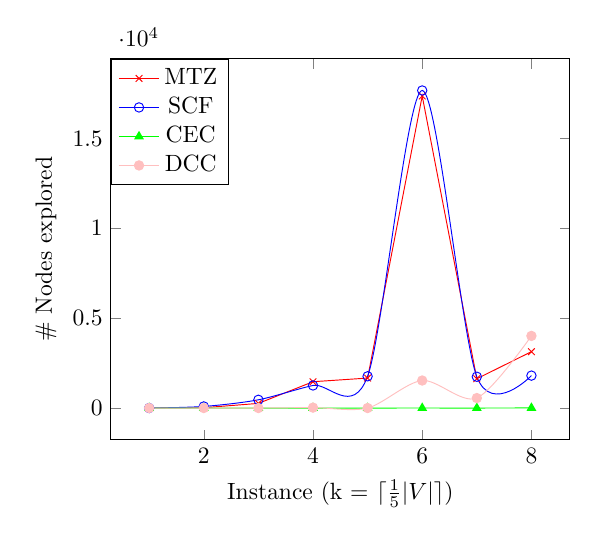
\begin{tikzpicture}[scale=0.85] 
\begin{axis}[ xlabel={Instance (k = $\lceil \frac{1}{5} |V| \rceil$)}, ylabel=\# Nodes explored=log, legend style={at={(0,1)},anchor=north west}] 
\addplot[color=red,mark=x] coordinates {(1,0.0) (2,19.0) (3,258.0) (4,1465.0) (5,1669.0) (6,17374.0) (7,1631.0) (8,3138.0)};
\addplot[smooth,color=blue,mark=o] coordinates {(1,0.0) (2,89.0) (3,459.0) (4,1257.0) (5,1767.0) (6,17679.0) (7,1743.0) (8,1805.0)};
\addplot[smooth,color=green,mark=triangle*] coordinates {(1,0) (2,0) (3,0) (4,0) (5,0) (6,1) (7,0) (8,6)};
\addplot[smooth,color=pink,mark=*] coordinates {(1,0) (2,0) (3,0) (4,24) (5,0) (6,1532) (7,555) (8,4016)};

\legend{MTZ, SCF, CEC, DCC}
\end{axis} 
\end{tikzpicture}
\end{minipage}
\hfill
\begin{minipage}{0.4\textwidth}
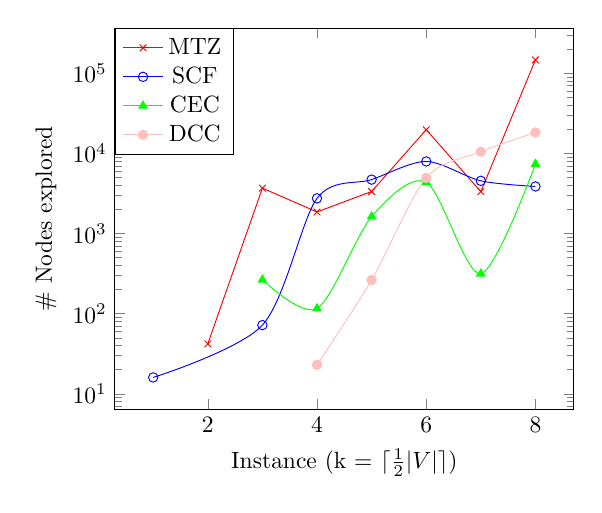
\begin{tikzpicture}[scale=0.85] 
\begin{axis}[ xlabel={Instance (k = $\lceil \frac{1}{2} |V| \rceil$)}, ylabel=\# Nodes explored, ymode=log, legend style={at={(0,1)},anchor=north west}] 
\addplot[color=red,mark=x] coordinates {(1,0.0) (2,42.0) (3,3687.0) (4,1859.0) (5,3348.0) (6,19768.0) (7,3337.0) (8,146821.0)};
\addplot[smooth,color=blue,mark=o] coordinates {(1,16.0) (2,0.0) (3,72.0) (4,2750.0) (5,4709.0) (6,7934.0) (7,4548.0) (8,3872.0)};
\addplot[smooth,color=green,mark=triangle*] coordinates {(1,0) (2,0) (3,265) (4,116) (5,1625) (6,4369) (7,315) (8,7362)};
\addplot[smooth,color=pink,mark=*] coordinates {(1,0) (2,0) (3,0) (4,23) (5,263) (6,4949) (7,10490) (8,18222)};


\legend{MTZ, SCF, CEC, DCC}
\end{axis} 
\end{tikzpicture}
\end{minipage}
\caption{Number of explored nodes for different formulations} \label{plot:nodes}
\end{figure}

\begin{figure}
\begin{minipage}{0.4\textwidth}
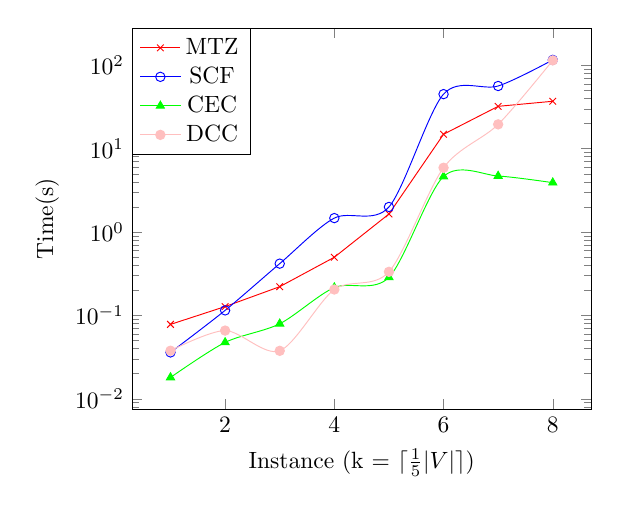
\begin{tikzpicture}[scale=0.85] 
\begin{axis}[ xlabel={Instance (k = $\lceil \frac{1}{5} |V| \rceil$)}, ylabel=Time(s), ymode=log, legend style={at={(0,1)},anchor=north west}] 
\addplot[color=red,mark=x] coordinates {(1,0.07802057266235352) (2,0.12757420539855957) (3,0.22100543975830078) (4,0.4982266426086426) (5,1.644547462463379) (6,14.874151229858398) (7,32.16856336593628) (8,36.99395775794983)}; 
\addplot[smooth,color=blue,mark=o] coordinates {(1,0.03599429130554199) (2,0.11484718322753906) (3,0.4177205562591553) (4,1.468893051147461) (5,1.9977211952209473) (6,45.048290729522705) (7,56.404672622680664) (8,115.92533326148987)};
\addplot[smooth,color=green,mark=triangle*] coordinates {(1,0.0180208683013916) (2,0.04742002487182617) (3,0.0793759822845459) (4,0.21576333045959473) (5,0.2859799861907959) (6,4.632004976272583) (7,4.696310520172119) (8,3.908022880554199)};
\addplot[smooth,color=pink,mark=*] coordinates {(1,0.03771710395812988) (2,0.06578278541564941) (3,0.037607669830322266) (4,0.2044692039489746) (5,0.3331305980682373) (6,5.901184797286987) (7,19.555060625076294) (8,114.4845073223114)};

\legend{MTZ, SCF, CEC, DCC}
\end{axis} 
\end{tikzpicture}
\end{minipage}
\hfill
\begin{minipage}{0.4\textwidth}
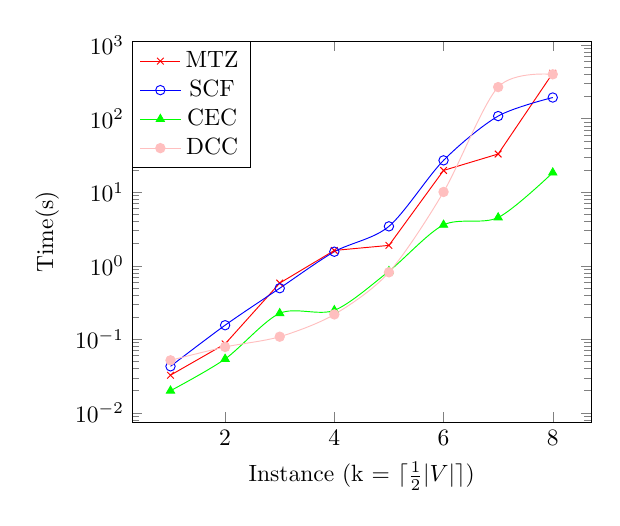
\begin{tikzpicture}[scale=0.85] 
\begin{axis}[ xlabel={Instance (k = $\lceil \frac{1}{2} |V| \rceil$)}, ylabel=Time(s), ymode=log, legend style={at={(0,1)},anchor=north west}] 
 \addplot[color=red,mark=x] coordinates {(1,0.03252410888671875) (2,0.0865168571472168) (3,0.5808014869689941) (4,1.6151392459869385) (5,1.8911528587341309) (6,19.76146149635315) (7,33.05476498603821) (8,414.95961332321167)};
 \addplot[smooth,color=blue,mark=o] coordinates {(1,0.04291081428527832) (2,0.15539121627807617) (3,0.4948270320892334) (4,1.5517733097076416) (5,3.432373523712158) (6,27.087477684020996) (7,108.3318018913269) (8,193.72209477424622)};
 \addplot[smooth,color=green,mark=triangle*] coordinates {(1,0.01998138427734375) (2,0.053990840911865234) (3,0.225569486618042) (4,0.24762582778930664) (5,0.8429348468780518) (6,3.591141939163208) (7,4.52320122718811) (8,18.430423259735107)};
\addplot[smooth,color=pink,mark=*] coordinates {(1,0.051819562911987305) (2,0.07871580123901367) (3,0.10845828056335449) (4,0.21785974502563477) (5,0.8141748905181885) (6,10.072609186172485) (7,268.6194157600403) (8,400.20856261253357)};

\legend{MTZ, SCF, CEC, DCC}
\end{axis} 
\end{tikzpicture}
\end{minipage}
\caption{Running times for different formulations} \label{plot:runtimes}
\end{figure}



\begin{figure}
\begin{minipage}{0.4\textwidth}
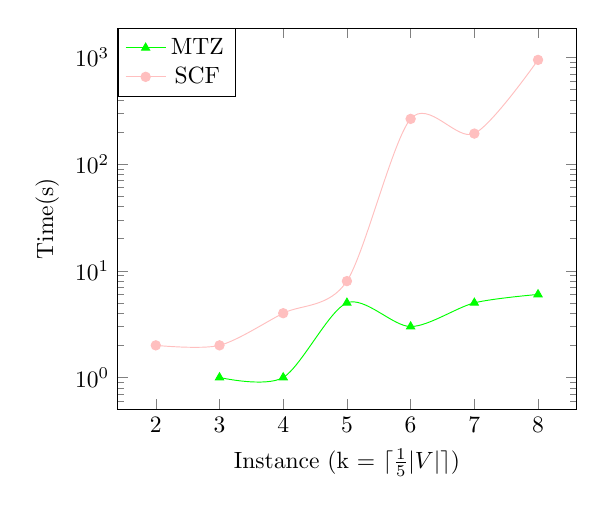
\begin{tikzpicture}[scale=0.85] 
\begin{axis}[ xlabel={Instance (k = $\lceil \frac{1}{5} |V| \rceil$)}, ylabel=Time(s), ymode=log, legend style={at={(0,1)},anchor=north west}] 
\addplot[smooth,color=green,mark=triangle*] coordinates {(1,0) (2,0) (3,1) (4,1) (5,5) (6,3) (7,5) (8,6)};
\addplot[smooth,color=pink,mark=*] coordinates {(1,0) (2,2) (3,2) (4,4) (5,8) (6,265) (7,193) (8,946)};

\legend{MTZ, SCF, CEC, DCC}
\end{axis} 
\end{tikzpicture}
\end{minipage}
\hfill
\begin{minipage}{0.4\textwidth}
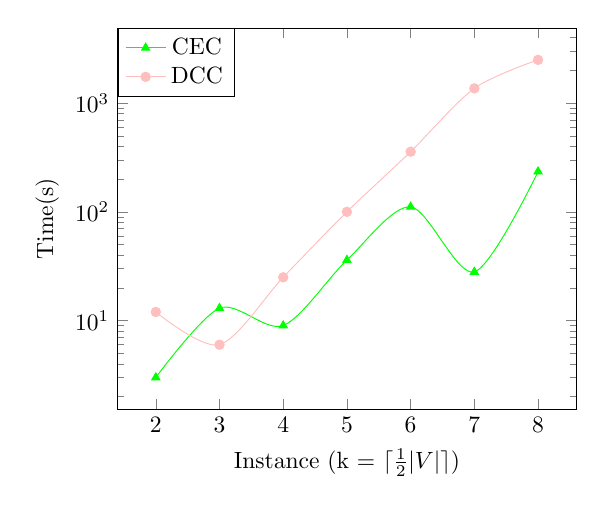
\begin{tikzpicture}[scale=0.85] 
\begin{axis}[ xlabel={Instance (k = $\lceil \frac{1}{2} |V| \rceil$)}, ylabel=Time(s), ymode=log, legend style={at={(0,1)},anchor=north west}] 
\addplot[smooth,color=green,mark=triangle*] coordinates {(1,0) (2,3) (3,13) (4,9) (5,36) (6,111) (7,28) (8,234)};
\addplot[smooth,color=pink,mark=*] coordinates {(1,0) (2,12) (3,6) (4,25) (5,100) (6,357) (7,1364) (8,2491)};


\legend{CEC, DCC}
\end{axis} 
\end{tikzpicture}
\end{minipage}
\caption{Number of violations added for different formulations} \label{plot:ineq}
\end{figure}



\end{document}
